\paragraph{}
Un système de gestion des informations géotechiques s'avère incontournable
dans un environnement de géoscience. Beaucoup d'universités et d'entreprises 
privées ainsi que l'état dans certains pays à travers le monde se sont déjà 
penchés sur la question. 
\paragraph{}
Les résutats divergent sur quelques détails à propos des technologies utilisées mais 
l'objectif est généralement le même: 
constituer une base de données renseignée regroupant tous les points (sondages, essais
in situ ou en laboratoire) améliorant la connaissance des caractéristiques géomécaniques des
formations d'une zone.
Par exemple, dans les Caraïbes, plus précisement sur l'Ile de Cayenne, un tel système a permis
de mieux appréhender les types de problèmes
spécifiques au site, et donc de mieux dimensionner les campagnes de reconnaissance
géotechniques, aussi bien sur le plan technique que financier
\cite{Cayenne}.
\par
L'une des faiblesses de certains projets est l'utilisation des outils de Microsoft
qui ne semblent pas assez 
adéquats. Ils sont trop génériques, ce qui empêche un stockage intelligent des données géotechniques
\cite{antoljak2012subsurface}.

%......................

\paragraph{}D'autres se basent de pŕeférence sur la Conception d'une architecture d'information 
géotechnique à l'aide de services Web
\cite{zimmermann2003design}.
Cette architecture d'information a été implémentée à Los Angeles afin de permettre les échanges 
d'informations géotechniques accessibles pour tous. Les avantages apportés par une telle 
application pourraient tant se sentir pour des études concernant les risques sismiques que pour 
une meilleure approche lors des estimations effectuées par des compagnies d'assurance. 

\paragraph{}
Au Canada, plusieurs projets identiques ont vu le jour, notemment l'élabora\-tion d'une base 
de données géoscientifiques dans le but d’aider à la finalisation de la 
cartographie des dépôts en surface et en subsurface
\cite{russell1996regional}.

%............................

\paragraph{}
En 2011, un séisme a frappé la région de Canterbury (Nouvelle-Zélande). Une base de données en ligne a été développée pour
la reconstruction de Christchurch à la suite du tremblement de terre:
La base de données géotechniques de Canterbury (CGD). Elle
a été conçu comme un référentiel consultable pour le partage d'informations géotechniques existantes et nouvelles
ainsi que des applications géotechniques de soutien pour les autorisations de construction. En mars
2015, la base de données contient plus de 18000 enregistrements d'essais de pénétration de cône, 4000 forages, 1000
piézomètres accompagnés de registres de surveillance des eaux souterraines, 6000 enregistrements de tests de laboratoire
plus d'autres données. 

\par
Le CGD a été conçu comme un référentiel consultable pour les informations géotechniques existantes et nouvelles
ainsi que des applications géotechniques de soutien pour les autorisations de construction et de ressources. Tandis que
les données sont principalement utilisées pour la conception géotechnique de l'amélioration du sol, la fondation du bâtiment
réparations, fondations de nouveaux bâtiments et conception géotechnique pour les réparations d'infrastructures, il peut
également être utilisé à des fins plus stratégiques telles que l'aide à la récupération pour de futurs
catastrophes naturelles, augmentation de la résilience d'autres régions de la Nouvelle-Zélande.
\cite{scott2015benefits}


\begin{figure}[t]
\centering
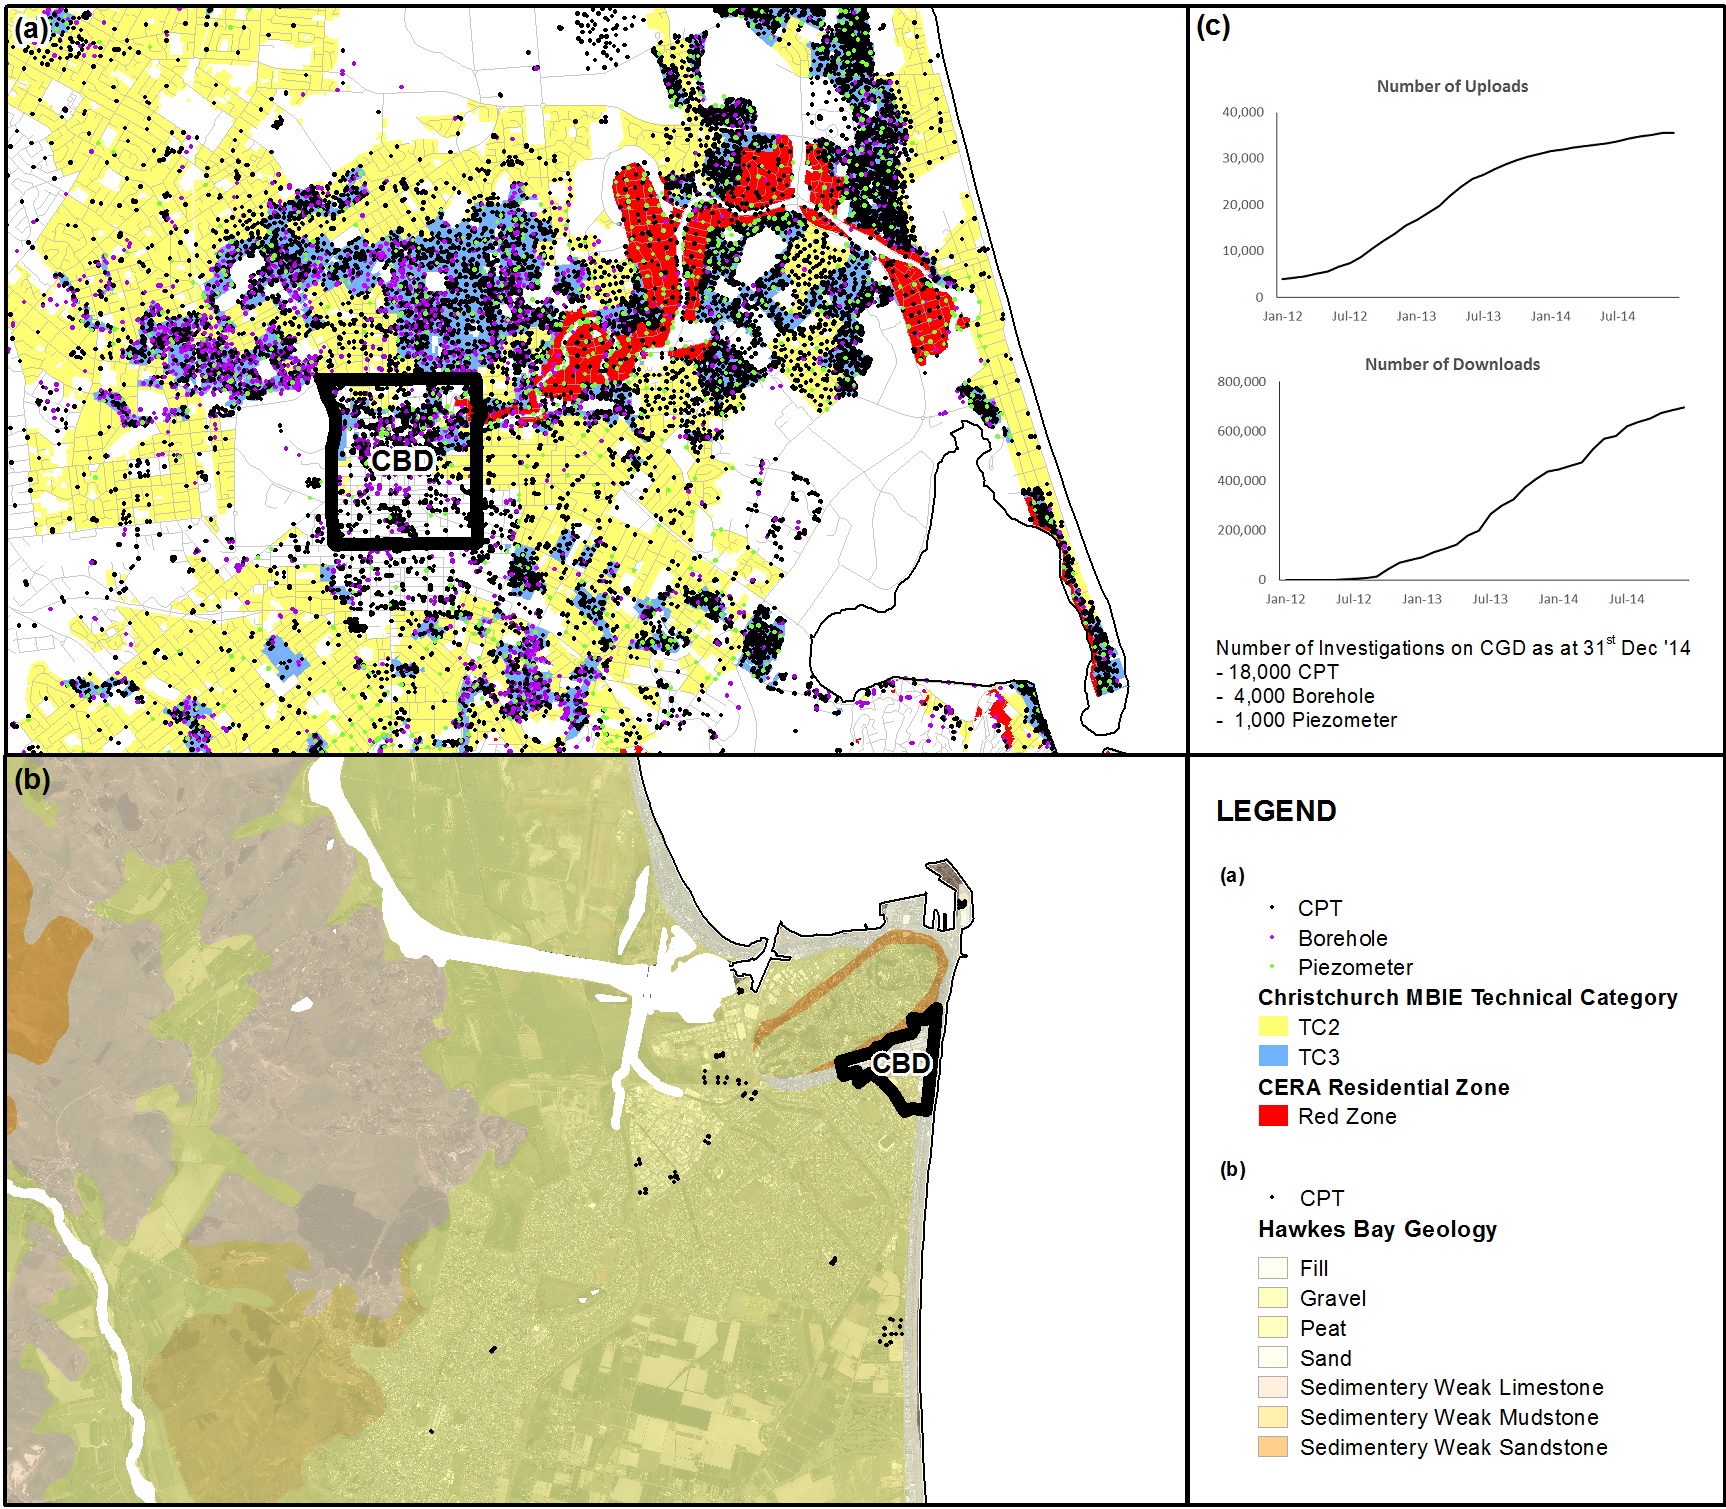
\includegraphics[width=1\textwidth]{cgd.png}
\caption{Visualisation des résultats de la base de données de Canterbury.}
\end{figure}

%............................

\paragraph{}
L'Afrique ne fait pas exception à la liste des multiples endroits ayant adopté l'idée
de concevoir une base do données géotechniques.
Par exemple, celle de la ville de Tunis (Tunisie) est orientée vers la cartographie géotechnique.
\par
Le modèle choisi a permis, après une analyse
pré1iminaire très importante, une description globale et
totale de toutes les données géologiques et géotechniques collectées sur le site de Tunis. I1
assure, de plus, une indépendance physique et logique, un partage des données (une même donnée accessible  
par plusieurs programmes), une non redondance des données, une non codification des
données géologiques, une grande facilité des relations
entre fichiers indépendants, une intégrité (validité)
totale des données. 
\textit{S'y ajoutent une souplesse remarquable d'interrogation de TUNIS-DATA-BANK
assurée par l'emploi d'un langage d'interrogation spécifique et l'utilisation des opérateurs et des connecteurs
logiques, une automatisation totale des tâches de la
phase de la manipulation de la base de données et une
sécurité totale des fichiers.}
\cite{tunis}

%..................

\paragraph{}
L’implémentation de tous ces SIG par des organismes internationaux résulte à des données considérées 
comme étant le système d’archivage officiel dans leur domaine de spécialité.
Le rythme de migration de ces données dans le SIG Web connait une croissance exponentielle. 
\par
Avec son mouvement vers le cloud et sur le Web, son intégration à l'information 
en temps réel via l'Internet des objets, le SIG est devenu une plateforme 
pertinente pour presque toutes les activités humaines - un système nerveux de 
la planète. Alors que notre pays est confronté au problèmes de gestion et de vulgarisation 
des données géotechiques, les SIG joueront un rôle de plus 
en plus important et 
fourniront un moyen de communiquer des solutions en utilisant le langage commun de 
la cartographie.